\chapter*{Introduction}
\renewcommand{\thefigure}{I.\arabic{figure}}
\addcontentsline{toc}{chapter}{Introduction}

Genetic information determines the constitution and function of the cells. However, genetically identical cells show differences, such as cells from our skin and our neurons. This is explained because there are mechanisms of gene regulation that determine the level of expression of each gene. Cells differentiate because they are expressing a different set of genes at different levels. These levels of expression respond e.g. to environmental signals that modify certain proteins called transcription factors whose function is to activate or repress the expression of certain gene or group of genes.

Transcription factors are also codified by certain gene, that may also be regulated by other transcription factor and external signals. A gene circuit is a group of genes, together with the external signals that affect them, that develops certain function in an organism and are connected by mechanisms such as the explained above.

The chemical reactions that regulate gene expression are, at a fundamental level, collisions between diffusing molecules that occur randomly. It is surprising how all these random chemical reactions are able to determine such complex and synchronized patterns in living beings. There must be sophisticated mechanisms in the genetic circuits that allow them to work properly regardless of the presence of noise \cite{kaern05} \cite{raj08}.

It has been observed that even clonal populations under the same environmental conditions have very different levels of expressions \cite{elowitz02} \cite{pedraza05}. Fig. \ref{fig:int-noise1} show the level of expression of genes, measured by flourescence, of genetically identical cells under the same conditions. The expression of each gene is proportional to the intensity of some specific color. Thus, the variability in the intensities of each color among cells show that genes are expressed at different levels. These evidences have shown that noise is inherent to biological systems and thus it is important to study it.

\begin{figure}[H]
  \centering
  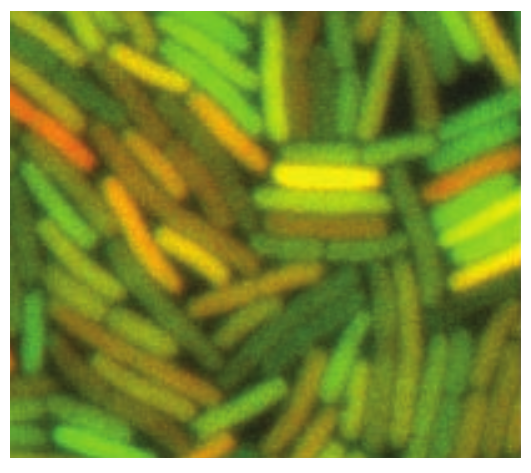
\includegraphics[width=15cm]{int-noise1}
  \caption[Examples of noise in gene expression]{\label{fig:int-noise1}Examples of noise in gene expression for clonal population under identical environmental conditions. (Left) An image taken by fluoresence microscopy of a population of bacteria. The large variation in the colors between the cells shows how noisy are the levels of the proteins. (Right) Scatter of the levels of expression, measured as fluorescence counts of two different genes. Each point represent an individual cell and the red lines mark the average. The levels of expression show huge variations relative to the average. From \cite{elowitz02} (left) and \cite{pedraza05} (right).}
\end{figure}

Besides, some works have considered genetic circuits where noise plays an important role. In \cite{arkin98}, a genetic circuit that determines the mechanism by which the lambda phage virus infects the bacteria \textit{E. coli} is studied. Fig. \ref{fig:int-lambda} summarizes it. When the phage infects the bacteria and introduces its genetic material there are two possible pathways. In the lytic pathway, the virus uses the cell to replicate its DNA, produce many viruses and then kill the bacteria. In the lysogenic pathway the viral DNA is inserted into the bacterial chromosome and replicated together with the bacterial DNA. If the virus is in the lysogenic phase, certain conditions can induce it to enter the lytic phase.

It turns out that the virus decides randomly which pathway to follow with probabilities that are weighted by conditions such as the ratio between viruses and bacteria and stress signals. This is more efficient because if all the phages take the lytic path, the entire population of bacteria would die and the viruses would not be able to replicate anymore. It is also inefficient for all the viral DNA to be hidden in the bacterial chromosome. Since each virus chooses its pathway randomly, diversity is introduced in the population. Therefore, evolution has designed this circuit to take advantage of noise \cite{arkin98}.

\begin{figure}[H]
  \centering
  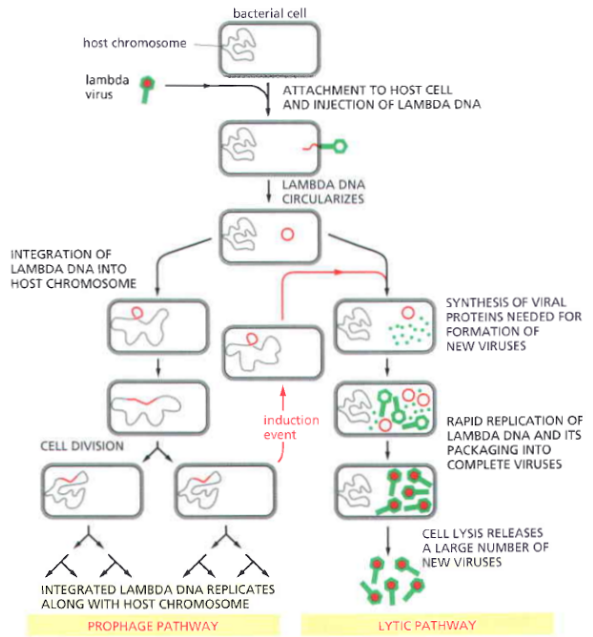
\includegraphics[width=13cm]{int-lambda}
  \caption[Life cycle of lambda phage]{\label{fig:int-lambda} Life cycle of lambda phage. When its DNA is injected into the cell it takes either the lytic or the prophage (or lysogenic) pathway. If the virus is in the lysogenic phase, it can switch back to the lytic phase. From \cite{alberts08}.}
\end{figure}

Other aspect in which noise plays an important role is on the adaptation to changing environments. For each environment there is an optimal phenotype. If the environmental conditions were fixed, the best strategy for a population would be to express the optimal phenotype. However, the external conditions may vary randomly and with an uncertain frequence. If cells synchronize their phenotypes with the changing environments, they would need to sense regularly their surroundings and this would have a high energetic cost. The less costly strategy is choosing the phenotype randomly, without performing any measurement. What actually happens is a combination of both strategies. Cells choose randomly between phenotypes with a higher bias for the phenotype that corresponds to the measured environment. Besides, the precision at the measurement of the environment can be regulated up to a limit and it is chosen according the relation with the energetic cost it implies (see fig. \ref{fig:int-environments1}). This strategy is advantageous because it lowers the energetic cost of precise sensing and also allows the population to be prepared for sudden changes in the environment \cite{kussell05}.

\begin{figure}[H]
  \centering
  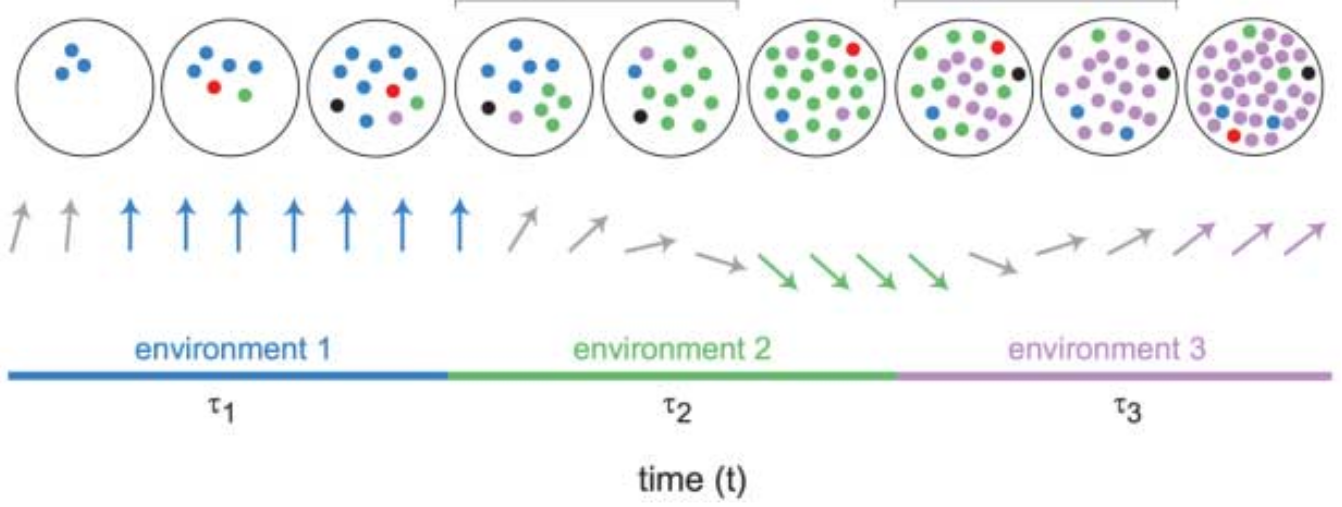
\includegraphics[width=13cm]{int-environments1}
  \caption[Stochastic switching strategy in fluctuating environments]{\label{fig:int-environments1}. Stochastic switching strategy in fluctuating environments. For each environment, represented as colors, there is an optimal phenotipic response represented with the same color as the environments. However, there are some cells that are in a phenotypic state different than the optimal. This is a good strategy when the environment changes randomly. From \cite{kussell05}.}
\end{figure}

On the other hand, there are biological functions that have to be very synchronized regardless of the noise present in the gene networks that regulate them. For example, cellular differentiation in developing embryos is determined by the level of expression of certain genes, which can fluctuate randomly. If fluctuations are not controlled, complex multicellular organisms would not develop properly.

The circuits that control cellular differentiation must be robust to noise, this means that they must be able to work properly regardless of its presence. Some of the strategies that ensure that important proteins are expressed exactly when needed and at precise levels include redundancy in genes, checkpoints in the cascade events and cooperation in the expression between individuals of a population (i.e. not every cell in the population needs to be active at the same rate) \cite{mcadams99}. Such strategies are used in many circuits that need to be reliable and precise.

From the previous examples it can be concluded that noise is clearly present in living systems and their circuits have evolved either to be robust to it, or to take advantage of it. This fact has inspired the development of mathematical models in the last years that have allowed us to elucidate how life works from a systemic approach. Besides, accuracy is usually very important when synthetic biological circuits are designed to perform some specific task. Then, stochastic models are useful as a prior test for their reliability.

In a pioneer work, Thattai and van Oudenaarden \cite{thattai01} made a linearized model for intrinsic noise in the amounts of RNA and proteins that can be applied to some basic gene circuits. Also, Pedraza and van Oudenaarden \cite{pedraza05} developed a model that includes extrinsic noise and showed how fluctuations are propagated through a cascade of regulation. Most recent models have focused in other aspects that could produce noise. For instance, the bursting in the production of the molecules involved in gene expression, their senescence \cite{pedraza08}, and the partition of molecules during cell division \cite{huh11a} \cite{huh11b}. One of the most important conclusions of these works is that when considering different factors, the behavior of noise is similar. Therefore, by studying only the fluctuations in concentrations it is very difficult to know the mechanisms that produce them.

In the next chapter we make a brief review of some of the basic concepts that are used in the models of gene expression. Then, we explain with detail the models along with the mathematical tools applied in them.

\renewcommand{\thefigure}{\arabic{chapter}.\arabic{section}.\arabic{figure}}
